\documentclass{beamer}
\usepackage{graphicx}
\usepackage{xcolor}
\usepackage{tikz}

% 自定义颜色
\definecolor{purpleblue}{RGB}{80, 80, 180}
\definecolor{lightgray}{RGB}{230, 230, 230}
\definecolor{novelPurple}{RGB}{98, 54, 255} 
\definecolor{darkgray}{RGB}{50, 50, 50}

% 主题设置
\usetheme{Madrid}  
\usecolortheme{dolphin} 

% 设置字体（移除 fontspec，确保 pdfLaTeX 兼容）
\setbeamerfont{title}{size=\Large,series=\bfseries}
\setbeamerfont{frametitle}{size=\LARGE,series=\bfseries}
\setbeamercolor{frametitle}{fg=white, bg=novelPurple}
\setbeamercolor{title}{fg=white, bg=purpleblue}

% 封面信息
\title[SAT Unit 2.2 Quadratic Function]{\textbf{SAT Unit 2.2\\ Quadratic function}}
\author{\textbf{Jack Zeng}}
\institute{\textcolor{white}{\textbf{Novel Prep}}}
\date{\today} 

\begin{document}

% --- Title Slide ---
\begin{frame}
    \titlepage
    \vfill
    \begin{flushright}
        \textcolor{purpleblue}{\Huge \textbf{Novel Prep}}
    \end{flushright}
\end{frame}


\begin{frame}
    \begin{tikzpicture}[remember picture, overlay]

        \shade[top color=softPurple, bottom color=softGray] 
            (current page.north west) rectangle (current page.south east);

        \fill[white, opacity=0.3] (current page.center) circle (4cm);
        

        \node[align=center] at (current page.center) {
            {\Huge\bfseries\textcolor{purpleblue}{Novel Prep}} \\[0.5cm]
            {\Large\itshape\textcolor{lightText}{Excellence in SAT Prep}}
        };
        \foreach \x in {1,2,3,4,5} {
            \fill[purpleblue, opacity=0.2] (rand*10-5, rand*7-3.5) circle (0.1+\x*0.05);
        }
        ;
    \end{tikzpicture}
\end{frame}

\begin{frame}{Overview}
    \tableofcontents
\end{frame}


% Slide 2: Introduction to Parabolas
\begin{frame}{\textbf{Parabolas}}
    A parabola is a symmetric curve that satisfies a quadratic function. Below are different forms of its equation and key properties.
\end{frame}

\begin{frame}
\section{Different Forms of a Parabola}
    \begin{tikzpicture}[remember picture, overlay]

        \shade[top color=softPurple, bottom color=softGray] 
            (current page.north west) rectangle (current page.south east);

        \fill[white, opacity=0.3] (current page.center) circle (4cm);
        

        \node[align=center] at (current page.center) {
            {\LARGE\bfseries\textcolor{purpleblue}{Different Forms of a Parabola}} \\[0.5cm]
            {\Large\itshape\textcolor{lightText}{Excellence in SAT Prep}}
        };
        \foreach \x in {1,2,3,4,5} {
            \fill[purpleblue, opacity=0.2] (rand*10-5, rand*7-3.5) circle (0.1+\x*0.05);
        }
        ;
    \end{tikzpicture}
\end{frame}

% Slide 3: Different Forms of a Parabola
\begin{frame}{\textbf{Standard Form}}
    \textbf{Standard Form:}
    \[
        f(x) = ax^2 + bx + c
    \]
    where:
    \begin{itemize}
        \item \( a \) determines the direction and width of the parabola.
        \begin{itemize}
            \item If \( a > 0 \), the parabola opens \textbf{upward} (concave up).
            \item If \( a < 0 \), the parabola opens \textbf{downward} (concave down).
        \end{itemize}
        \item \( b \) affects the location of the vertex along the \( x \)-axis.
        \item \( c \) is the \( y \)-intercept.
    \end{itemize}

    \begin{center}
        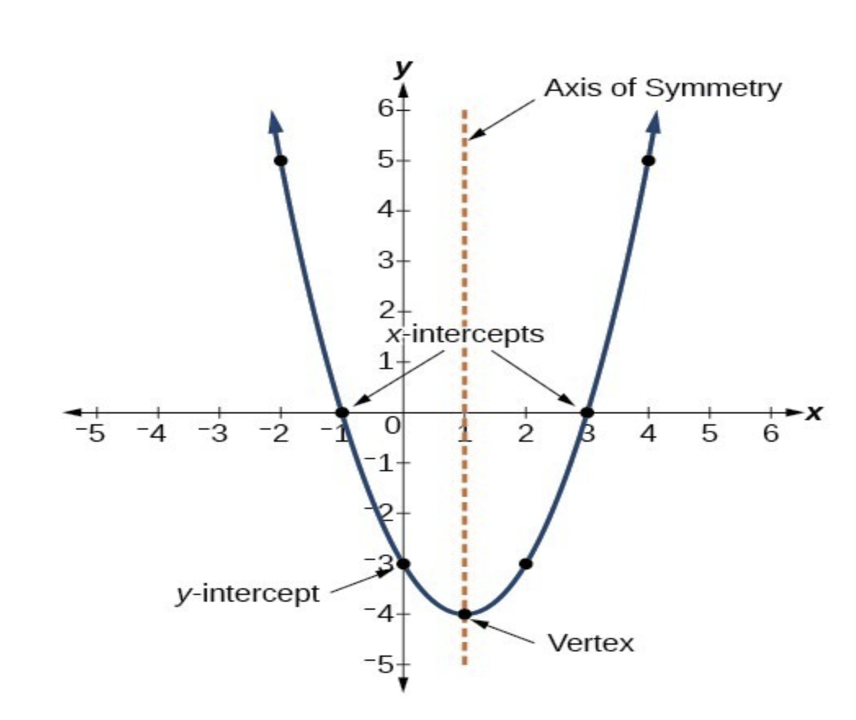
\includegraphics[width=0.4\linewidth]{E1.png}
    \end{center}
\end{frame}



\begin{frame}{\textbf{Vertex Form}}


    \textbf{Vertex Form:}
    \[
        f(x) = a(x - h)^2 + k
    \]
    where \( (h, k) \) is the vertex of the parabola.

    \begin{center}
    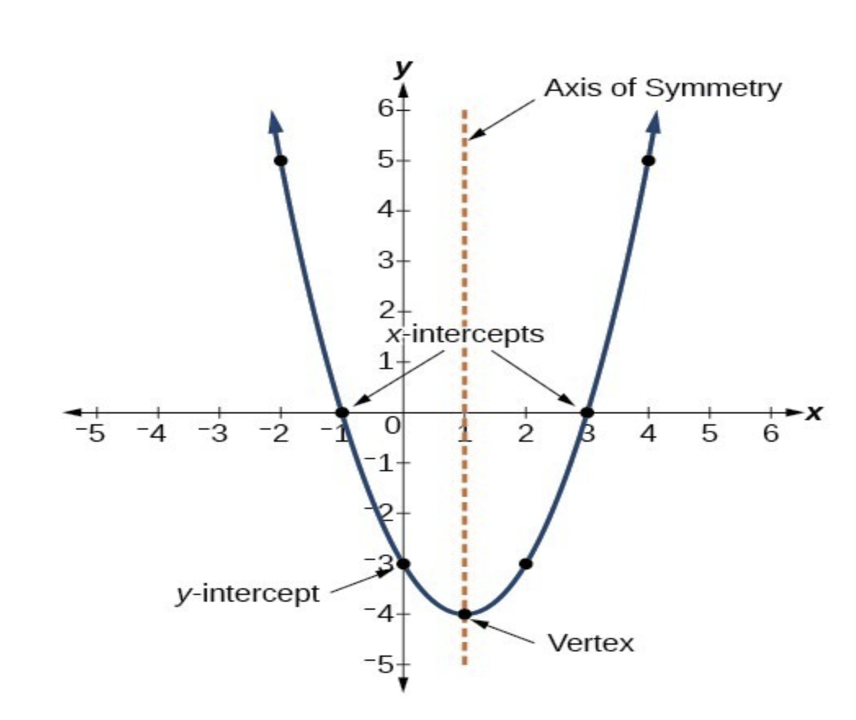
\includegraphics[width=0.5\linewidth]{E1.png}
\end{center}
\end{frame}


\begin{frame}{\textbf{Factored Form}}

    \textbf{Factored Form:}
    \[
        f(x) = a(x - m)(x - n)
    \]
    where \( m \) and \( n \) are the \( x \)-intercepts (roots) of the parabola.

    \begin{center}
    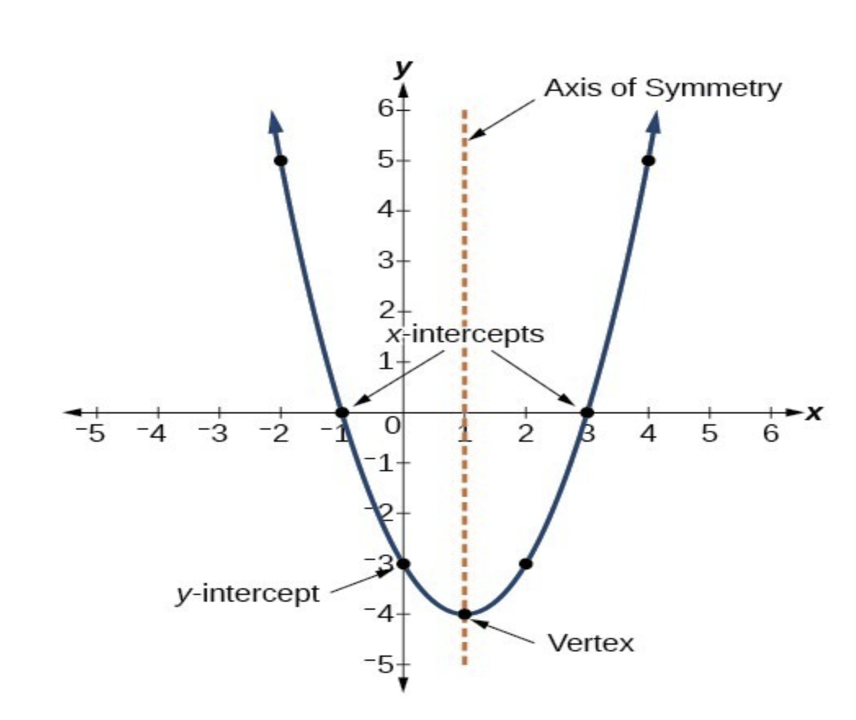
\includegraphics[width=0.5\linewidth]{E1.png}
\end{center}

\end{frame}

\begin{frame}{Question: Quadratic Function from Three Conditions}
\small
\textbf{Problem:}

A quadratic function $f(x)$ satisfies the following:

\begin{itemize}
    \item The vertex of the parabola is at $(3, -16)$.
    \item The graph passes through the point $(5, -12)$.
    \item One of the roots of $f(x)$ is $1$.
\end{itemize}

\vspace{0.3cm}
\textbf{Tasks:}
\begin{enumerate}
    \item Write the function in vertex form.
    \item Convert your function to standard form.
    \item Express the function in factored form.
\end{enumerate}
\end{frame}

\begin{frame}{Solution: Challenge Problem}
\small
\textbf{Step 1: Vertex Form}

\[
f(x) = a(x - 3)^2 - 16
\]
Plug in $(5, -12)$ to solve for $a$:
\[
-12 = a(5 - 3)^2 - 16 \Rightarrow -12 = 4a - 16 \Rightarrow 4a = 4 \Rightarrow a = 1
\]

\[
\Rightarrow f(x) = (x - 3)^2 - 16
\]

\vspace{0.3cm}
\textbf{Step 2: Standard Form}

\[
f(x) = x^2 - 6x + 9 - 16 = x^2 - 6x - 7
\]

\vspace{0.3cm}
\textbf{Step 3: Factored Form}

\[
f(x) = (x - 7)(x + 1)
\]
(One root is $1$, so the other must be $7$ since sum of roots = $6$)

\end{frame}




\begin{frame}
\section{Properties of a Parabola}
    \begin{tikzpicture}[remember picture, overlay]

        \shade[top color=softPurple, bottom color=softGray] 
            (current page.north west) rectangle (current page.south east);

        \fill[white, opacity=0.3] (current page.center) circle (4cm);
        

        \node[align=center] at (current page.center) {
            {\LARGE\bfseries\textcolor{purpleblue}{ Key Properties of a Parabola}} \\[0.5cm]
            {\Large\itshape\textcolor{lightText}{Excellence in SAT Prep}}
        };
        \foreach \x in {1,2,3,4,5} {
            \fill[purpleblue, opacity=0.2] (rand*10-5, rand*7-3.5) circle (0.1+\x*0.05);
        }
        ;
    \end{tikzpicture}
\end{frame}



% Slide 4: Key Properties of a Parabola
\begin{frame}{\textbf{Vertex}}

    \textbf{Standard Form:}
    \[
        f(x) = ax^2 + bx + c
    \]
    \textbf{Vertex:}
    \[
        x = \frac{-b}{2a}, \quad y = f\left(\frac{-b}{2a}\right)=\frac{4ac-b^2}{4a}
    \]
\begin{center}
    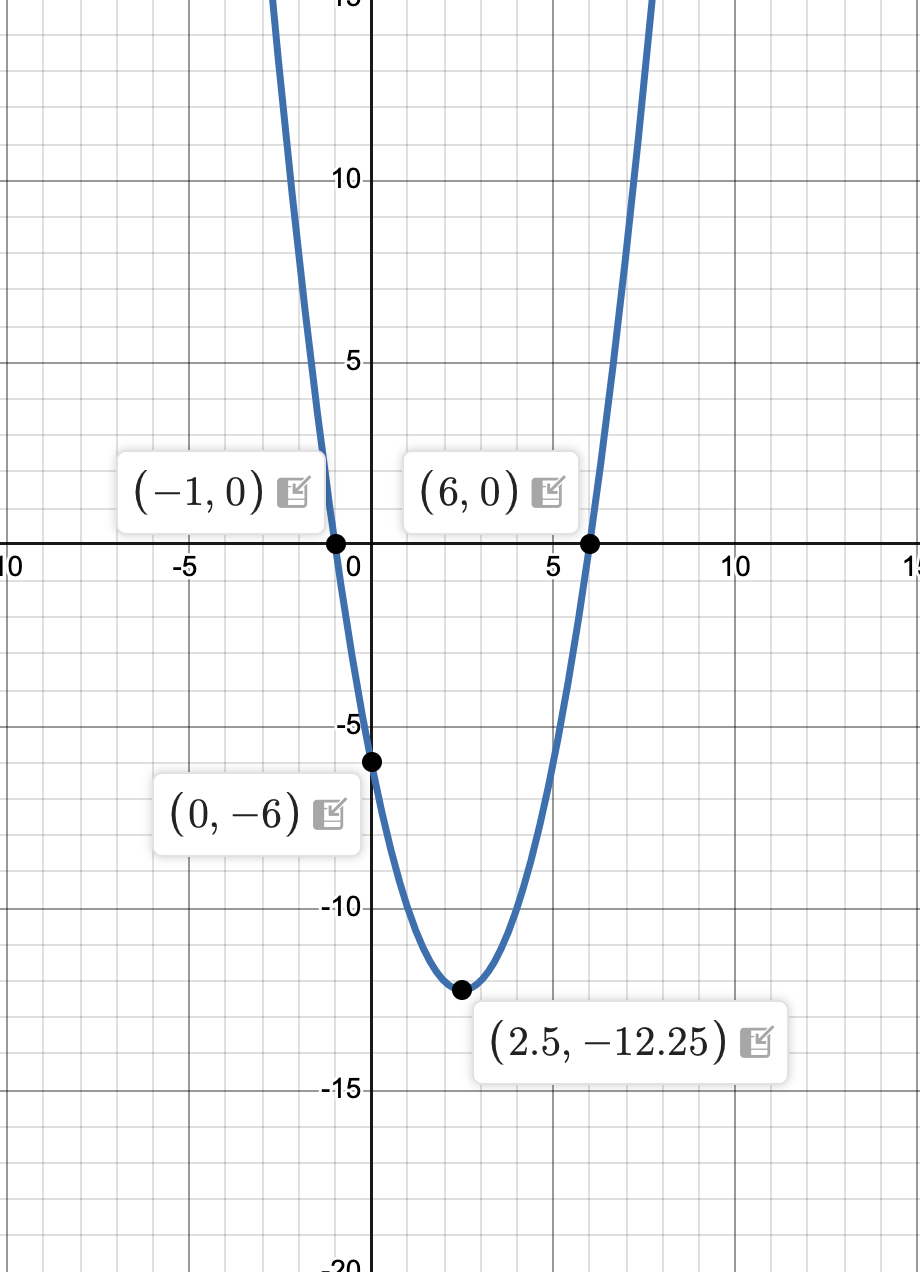
\includegraphics[width=0.35\linewidth]{E2.png}
\end{center}

\end{frame}

\begin{frame}{\textbf{Question: Minimum Value of Transformed Quadratic Function}}
    The function \( f(x) = 4x^2 + 64x + 262 \).  
    The function \( g \) is defined by:
    \[
    g(x) = f(x + 5)
    \]
    For what value of \( x \) does \( g(x) \) reach its minimum?

    \vspace{0.4cm}
    \textbf{Options:}
    \begin{enumerate}
        \item[A] \( -13 \)
        \item[B] \( -8 \)
        \item[C] \( -5 \)
        \item[D] \( -3 \)
    \end{enumerate}
\end{frame}

\begin{frame}{\textbf{Answer Explanation: Minimum of \( g(x) = f(x+5) \)}}
    \textbf{Correct Answer: \(\boxed{-13}\)}

    \vspace{0.2cm}
    \textbf{Step 1:} Find the vertex of the quadratic function  
    Since \( f(x) = ax^2 + bx + c \), the vertex is at:
    \[
    x = -\frac{b}{2a} = -\frac{64}{2(4)} = -8
    \]

    \textbf{So, the minimum of } \( f(x) \) occurs at \( x = -8 \)

    \vspace{0.3cm}
    \textbf{Step 2:} Apply the transformation to \( g(x) = f(x+5) \)  
    This is a horizontal shift \textbf{left by 5 units}.  
    So the minimum of \( g(x) \) occurs at:
    \[
    x + 5 = -8 \Rightarrow x = -13
    \]

    \vspace{0.2cm}
    \textbf{Final Answer:} \(\boxed{-13}\)
\end{frame}






% Slide 4: Key Properties of a Parabola
\begin{frame}{\textbf{Axis of Symmetry}}

    \textbf{Standard Form:}
    \[
        f(x) = ax^2 + bx + c
    \]
    \textbf{Axis of Symmetry:}
    \[
        x = \frac{-b}{2a}
    \]
\begin{center}
    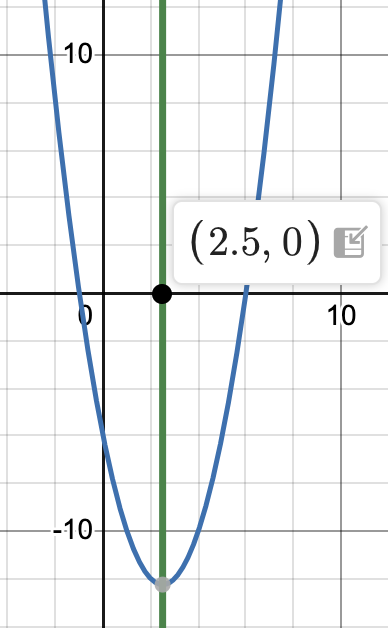
\includegraphics[width=0.3\linewidth]{E3.png}
\end{center}

\end{frame}

\begin{frame}{\textbf{Question: Minimum of Quadratic Function (Factored Form)}}
    The function is defined as:
    \[
    f(x) = (x - 14)(x + 19)
    \]
    For what value of \( x \) does \( f(x) \) reach its minimum?

    \vspace{0.4cm}
    \textbf{Options:}
    \begin{enumerate}
        \item[A] \( -266 \)
        \item[B] \( -19 \)
        \item[C] \( -\frac{33}{2} \)
        \item[D] \( -\frac{5}{2} \)
    \end{enumerate}
\end{frame}


\begin{frame}{\textbf{Answer Explanation: Minimum of } \( f(x) = (x - 14)(x + 19) \)}
    \textbf{Correct Answer: \(\boxed{D}\)}

    \vspace{0.1cm}
    \textbf{Step 1:} Use the axis of symmetry formula for a quadratic in factored form:
    \[
    x = \frac{r_1 + r_2}{2}
    \]
    where \( r_1 = 14 \), \( r_2 = -19 \)

    \[
    x = \frac{14 + (-19)}{2} = \frac{-5}{2} = -\frac{5}{2}
    \]

\end{frame}


\begin{frame}{\textbf{Question: Properties of a Quadratic Function}}
The function is given as:
\[
f(x) = ax^2 + 4x + c
\]
where \(a\) and \(c\) are constants. The parabola opens upward and it is also given that:
\begin{itemize}

    \item \(f(-9) = f(3)\)
\end{itemize}

What is the value of $a$?
\end{frame}


\begin{frame}{\textbf{Answer Explanation: Use of Symmetry and Vertex}}
We are told:
\[
f(x) = ax^2 + 4x + c
\quad \text{and} \quad f(-9) = f(3)
\]

\textbf{Step 1: Use symmetry of a parabola.}  
If \(f(-9) = f(3)\), then these points are symmetric about the vertex.

So, the axis of symmetry (i.e. x-value of vertex) is:
\[
x = \frac{-9 + 3}{2} = -3
\]

\textbf{Step 2: Use vertex formula to confirm.}  
The x-coordinate of the vertex of a quadratic is given by:
\[
x = \frac{-b}{2a}
\]
Here, \(f(x) = ax^2 + 4x + c\), so:
\[
\frac{-4}{2a} = -3 \Rightarrow a = \frac{2}{3}
\]


\end{frame}

\begin{frame}{Question}
In the $xy$-plane, a parabola has vertex $\left(\dfrac{7}{3}, -4\right)$ and intersects the $x$-axis at $(10, 0)$ and $(a, 0)$, where $a$ is a constant.

What is the value of $a$?

\begin{enumerate}
  \item[A)] $-10$
  \item[B)] $-\dfrac{23}{3}$
  \item[C)] $-\dfrac{19}{3}$
  \item[D)] $-\dfrac{16}{3}$
\end{enumerate}
\end{frame}

\begin{frame}{Answer}
We are given the vertex $\left(\dfrac{7}{3}, -4\right)$ and the $x$-intercepts $(10, 0)$ and $(a, 0)$. So the parabola has roots at $x = 10$ and $x = a$, and the vertex is at the midpoint of the roots.

Use midpoint formula:
\[
\frac{10 + a}{2} = \frac{7}{3}
\Rightarrow 10 + a = \frac{14}{3}
\Rightarrow a = \frac{14}{3} - 10 = \frac{14 - 30}{3} = -\frac{16}{3}
\]

\textbf{Correct answer:} D
\end{frame}


\begin{frame}{Question}
The function 
\[
f(x) = (x - 3)(x - k)
\]
is a quadratic, where $k$ are constants.

The graph of $y = f(x)$ in the $xy$-plane is a parabola with vertex $(5, -32)$. What is the value of $k$?

\begin{enumerate}
  \item[A)] 2
  \item[B)] 5
  \item[C)] 7
  \item[D)] 8
\end{enumerate}
\end{frame}



\begin{frame}{Answer}

c

\end{frame}







\begin{frame}
\section{Quadratic Formula(X-Intercept)}
    \begin{tikzpicture}[remember picture, overlay]

        \shade[top color=softPurple, bottom color=softGray] 
            (current page.north west) rectangle (current page.south east);

        \fill[white, opacity=0.3] (current page.center) circle (4cm);
        

        \node[align=center] at (current page.center) {
            {\LARGE\bfseries\textcolor{purpleblue}{Quadratic Formula(X-Intercept)}} \\[0.5cm]
            {\Large\itshape\textcolor{lightText}{Excellence in SAT Prep}}
        };
        \foreach \x in {1,2,3,4,5} {
            \fill[purpleblue, opacity=0.2] (rand*10-5, rand*7-3.5) circle (0.1+\x*0.05);
        }
        ;
    \end{tikzpicture}
\end{frame}

\begin{frame}{Discriminant of a Quadratic Equation}
\textbf{General Form of a Quadratic:}
\[
ax^2 + bx + c = 0
\]

\textbf{Discriminant Formula:}
\[
\Delta = b^2 - 4ac
\]

\textbf{Why is the discriminant important?}

\begin{itemize}
    \item Tells us how many and what type of solutions the quadratic equation has.
\end{itemize}

\textbf{Cases:}
\begin{itemize}
    \item $\Delta > 0$: Two distinct real solutions
    \item $\Delta = 0$: One real solution (a repeated root)
    \item $\Delta < 0$: No real solutions (complex roots)
\end{itemize}
\end{frame}

\begin{frame}{Graphical Meaning of the Discriminant}
\small
\textbf{How the Discriminant relates to the graph of} $y = ax^2 + bx + c$:

\begin{itemize}
    \item $\Delta > 0$: The parabola intersects the $x$-axis at \textbf{two points}.
    \item $\Delta = 0$: The parabola is \textbf{tangent} to the $x$-axis (one point of contact).
    \item $\Delta < 0$: The parabola does \textbf{not intersect} the $x$-axis.
\end{itemize}

\vspace{0.3cm}
\textbf{Implication:} You can \textit{predict} how many real solutions an equation has by simply analyzing its discriminant.


\begin{center}
    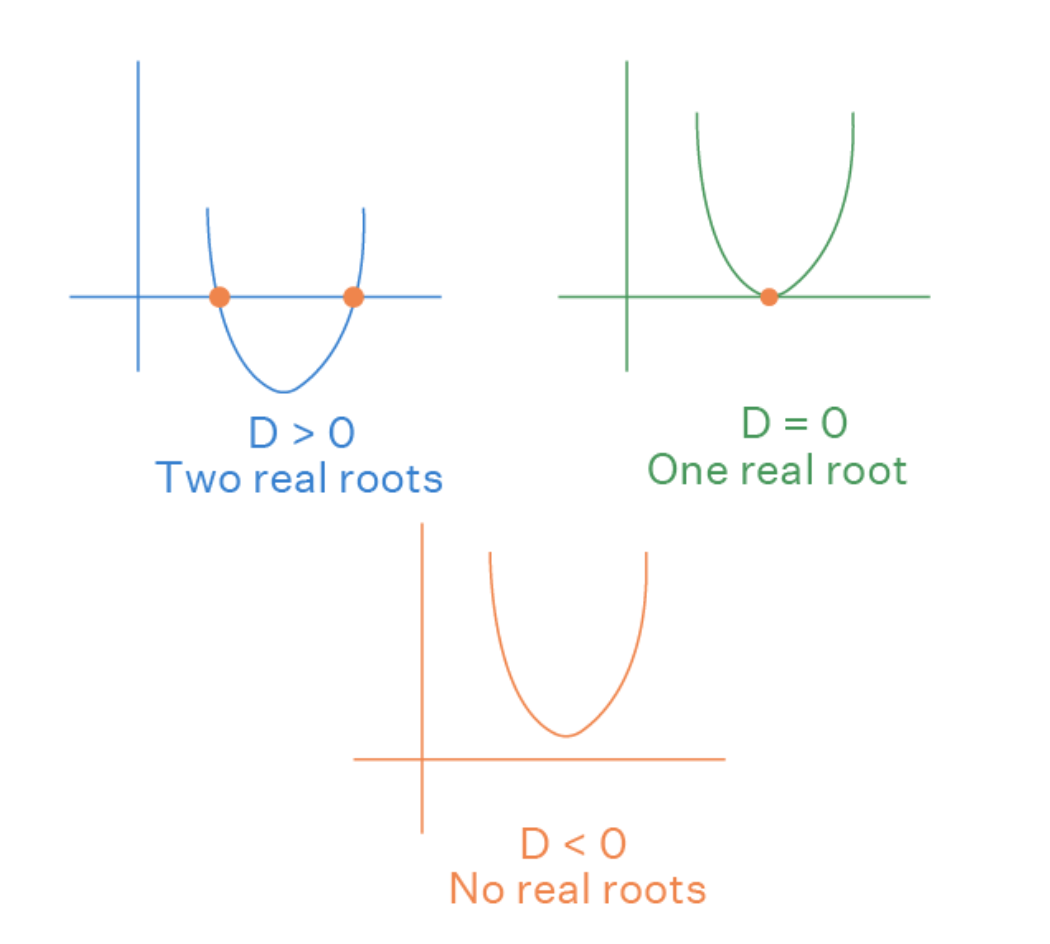
\includegraphics[width=0.45\linewidth]{E21.png}
\end{center}
\end{frame}


\begin{frame}{Question}
\[
2x^2 - 13x + 21 = 0
\]

How many distinct real solutions does the given equation have?

\begin{enumerate}
  \item[A)] Zero
  \item[B)] Exactly one
  \item[C)] Exactly two
  \item[D)] Infinitely many
\end{enumerate}
\end{frame}

\begin{frame}{Answer}
We are given the quadratic equation:
\[
2x^2 - 13x + 21 = 0
\]

Use the discriminant to determine the number of real solutions:
\[
\Delta = b^2 - 4ac = (-13)^2 - 4(2)(21) = 169 - 168 = 1
\]

Since $\Delta > 0$, the equation has two distinct real solutions.

\textbf{Correct answer:} C
\end{frame}



\begin{frame}{\textbf{Question: Discriminant and No Real Solutions}}
Consider the quadratic equation:
\[
x^2 - 34x + c = 0
\]
In the given equation, \(c\) is a constant. The equation has \textbf{no real solutions} if \(c > n\).  
What is the least possible value of \(n\)?


\end{frame}


\begin{frame}{\textbf{Answer Explanation: Using the Discriminant}}
\small
A quadratic equation \(ax^2 + bx + c = 0\) has:
\begin{itemize}
    \item \textbf{Two real solutions} if \(b^2 - 4ac > 0\)
    \item \textbf{One real solution} if \(b^2 - 4ac = 0\)
    \item \textbf{No real solution} if \(b^2 - 4ac < 0\)
\end{itemize}

\vspace{0.3cm}
In our equation:
\[
x^2 - 34x + c = 0 \quad \Rightarrow \quad a = 1, \quad b = -34, \quad c = c
\]

Compute the discriminant:
\[
\Delta = (-34)^2 - 4(1)(c) = 1156 - 4c
\]

Set discriminant to be less than 0:
\[
1156 - 4c < 0 \quad \Rightarrow \quad 4c > 1156 \quad \Rightarrow \quad c > 289
\]

Therefore, the equation has no real solutions when:
\[
c > 289 \quad \Rightarrow \boxed{n = 289}
\]
\end{frame}










\begin{frame}{The Quadratic Formula}
\textbf{To solve any quadratic equation:}
\[
ax^2 + bx + c = 0
\]

\textbf{Use the Quadratic Formula:}
\[
x = \frac{-b \pm \sqrt{b^2 - 4ac}}{2a}
\]

\textbf{Steps to Use the Formula:}
\begin{enumerate}
    \item Identify $a$, $b$, and $c$ from the equation.
    \item Plug the values into the formula.
    \item Simplify the square root (use the discriminant).
    \item Solve for both values using $+$ and $-$.
\end{enumerate}

\textbf{Note:} Always check the discriminant before solving to understand the type of roots.
\end{frame}


\begin{frame}{\textbf{Question: Quadratic Equation with Radical Solutions}}
    Consider the equation:
    \[
    2x^2 - 2 = 2x + 3
    \]
    Which of the following is a solution to the equation above?

    \vspace{0.3cm}
    \textbf{Options:}
    \begin{enumerate}
        \item[A] \(2\)
        \item[B] \(1 - \sqrt{11}\)
        \item[C] \(\frac{1}{2} + \sqrt{11}\)
        \item[D] \(\frac{1 + \sqrt{11}}{2}\)
    \end{enumerate}
\end{frame}

\begin{frame}{\textbf{Answer Explanation: Quadratic Equation with Radical Solutions}}
    \textbf{Correct Answer: \textcolor{novelGreen}{D: \( \frac{1 + \sqrt{11}}{2} \)}}

    \vspace{0.3cm}
    \textbf{Solution:}
    \begin{itemize}
        \item Start by rearranging the equation:
        \[
        2x^2 - 2 = 2x + 3 \Rightarrow 2x^2 - 2x - 5 = 0
        \]
        \item Use the quadratic formula:
        \[
        x = \frac{-(-2) \pm \sqrt{(-2)^2 - 4(2)(-5)}}{2(2)} = \frac{2 \pm \sqrt{4 + 40}}{4} = \frac{2 \pm \sqrt{44}}{4}
        \]
        \item Therefore, the solutions are:
        \[
        x = \frac{1 + \sqrt{11}}{2}, \quad x = \frac{1 - \sqrt{11}}{2}
        \]
    \end{itemize}

    \textbf{Final Answer:} \( \boxed{\frac{1 + \sqrt{11}}{2}} \)
\end{frame}



\begin{frame}{\textbf{Question: Solving a Quadratic Equation Involving Radicals}}
    Solve the quadratic equation:
    \[
    x^2 - 2x - 9 = 0
    \]
    One solution to the equation can be written in the form \(1 + \sqrt{k}\), where \(k\) is a constant.

    \vspace{0.3cm}
    What is the value of \(k\)?

    \vspace{0.5cm}
    \textbf{Options:}
    \begin{enumerate}
        \item[A] \(8\)
        \item[B] \(10\)
        \item[C] \(20\)
        \item[D] \(40\)
    \end{enumerate}
\end{frame}

\begin{frame}{\textbf{Answer Explanation: Solving a Quadratic Equation Involving Radicals}}
    \textbf{Correct Answer: \textcolor{novelGreen}{C: \(20\)}}

    \vspace{0.3cm}
    \textbf{Solution:}
    \begin{itemize}
        \item Use the quadratic formula:
        \[
        x = \frac{2 \pm \sqrt{(-2)^2 - 4(1)(-9)}}{2(1)} = \frac{2 \pm \sqrt{4 + 36}}{2} = \frac{2 \pm \sqrt{40}}{2}
        \]
        \item Simplify:
        \[
        x = \frac{2 \pm 2\sqrt{10}}{2} = 1 \pm \sqrt{10}
        \]
        \item One solution is \(1 + \sqrt{10}\), so we identify:
        \[
        \sqrt{k} = \sqrt{10} \Rightarrow k = 10
        \]
    \end{itemize}

    \textbf{Final Answer:} \( \boxed{10} \)
\end{frame}



\begin{frame}{\textbf{Question: Smallest Solution to a Radical Equation}}
Solve the equation:
\[
\sqrt{(x - 2)^2} = \sqrt{3x + 34}
\]
What is the \textbf{smallest solution} to the given equation?
\end{frame}


\begin{frame}{\textbf{Answer Explanation: Solving Radical Equation}}


Square both sides:
\[
(x - 2)^2 = 3x + 34
\Rightarrow x^2 - 4x + 4 = 3x + 34
\Rightarrow x^2 - 7x - 30 = 0
\Rightarrow (x - 10)(x + 3) = 0
\Rightarrow x = 10 \quad \text{or} \quad x = -3
\]

Now check for extraneous solutions by plugging into the original equation:

- For \(x = 10\):
\[
\sqrt{(10 - 2)^2} = \sqrt{3(10) + 34}
\Rightarrow \sqrt{64} = \sqrt{64} \quad \text{✅ valid}
\]

- For \(x = -3\):
\[
\sqrt{(-3 - 2)^2} = \sqrt{3(-3) + 34}
\Rightarrow \sqrt{25} = \sqrt{25} \quad \text{✅ valid}
\]

\textbf{Case 2:} \(-(x - 2) = \sqrt{3x + 34}\)

This will yield the same roots already considered since squaring removes signs.

\vspace{0.3cm}
\textbf{Final Answer:} \(\boxed{-3}\)
\end{frame}


\begin{frame}{\textbf{Question: Solving a Radical Equation}}
Solve the equation:
\[
\sqrt{2x + 6} + 4 = x + 3
\]
What is the solution set?

\textbf{Options:}
\begin{enumerate}
    \item[A.] \(\{-1\}\)
    \item[B.] \(\{5\}\)
    \item[C.] \(\{-1, 5\}\)
    \item[D.] \(\{0, -1, 5\}\)
\end{enumerate}
\end{frame}

\begin{frame}{\textbf{Answer Explanation: Solving Radical Equation}}
We start with the given equation:
\[
\sqrt{2x + 6} + 4 = x + 3
\]

Subtract 4 from both sides:
\[
\sqrt{2x + 6} = x - 1
\]

Now square both sides:
\[
2x + 6 = (x - 1)^2
\Rightarrow 2x + 6 = x^2 - 2x + 1
\]

Move all terms to one side:
\[
0 = x^2 - 4x - 5
\Rightarrow (x - 5)(x + 1) = 0
\Rightarrow x = 5 \quad \text{or} \quad x = -1
\]


\end{frame}

\begin{frame}{Answer Explanation: Solving Radical
Equation}
    \textbf{Check for extraneous solutions:}

For \(x = 5\):
\[
\sqrt{2(5) + 6} + 4 = \sqrt{16} + 4 = 4 + 4 = 8
\quad\text{and}\quad x + 3 = 8 \quad \Rightarrow \text{✅ valid}
\]

For \(x = -1\):
\[
\sqrt{2(-1) + 6} + 4 = \sqrt{4} + 4 = 2 + 4 = 6
\quad\text{and}\quad -1 + 3 = 2 \quad \Rightarrow \text{❌ not valid}
\]

\textbf{Final Answer:} \(\boxed{\{5\}}\)
\end{frame}


\begin{frame}
\section{System of the Equations)}
    \begin{tikzpicture}[remember picture, overlay]

        \shade[top color=softPurple, bottom color=softGray] 
            (current page.north west) rectangle (current page.south east);

        \fill[white, opacity=0.3] (current page.center) circle (4cm);
        

        \node[align=center] at (current page.center) {
            {\LARGE\bfseries\textcolor{purpleblue}{System of the Equations}} \\[0.5cm]
            {\Large\itshape\textcolor{lightText}{Excellence in SAT Prep}}
        };
        \foreach \x in {1,2,3,4,5} {
            \fill[purpleblue, opacity=0.2] (rand*10-5, rand*7-3.5) circle (0.1+\x*0.05);
        }
        ;
    \end{tikzpicture}
\end{frame}


\begin{frame}{What is a System of Equations?}
  \begin{itemize}
    \item A \textbf{system of equations} is a set of two or more equations with the same variables.
    \item The solution is the point(s) that make all equations true at the same time.
  \end{itemize}
  \vspace{1em}
  \textbf{Example:}
  \[
  \begin{cases}
  y = 2x + 1 \\
  y = -x + 4
  \end{cases}
  \]
  \vspace{0.5em}
  \textit{Find the value of $x$ and $y$ that satisfies both equations.}
\end{frame}

\begin{frame}{Solving by Graphing}
  \begin{itemize}
    \item Plot both equations into the Desmos.
    \item The intersection point is the solution to the system.
  \end{itemize}
  \[
  \begin{cases}
  y = x^2 \\
  y = 2x + 3
  \end{cases}
  \]
  \vspace{1em}
  \textbf{Graph to find the point(s) of intersection.}
  \pause
  \[
  \text{Solution: The two curves intersect at points where } x^2 = 2x + 3.
  \]

  \begin{center}
      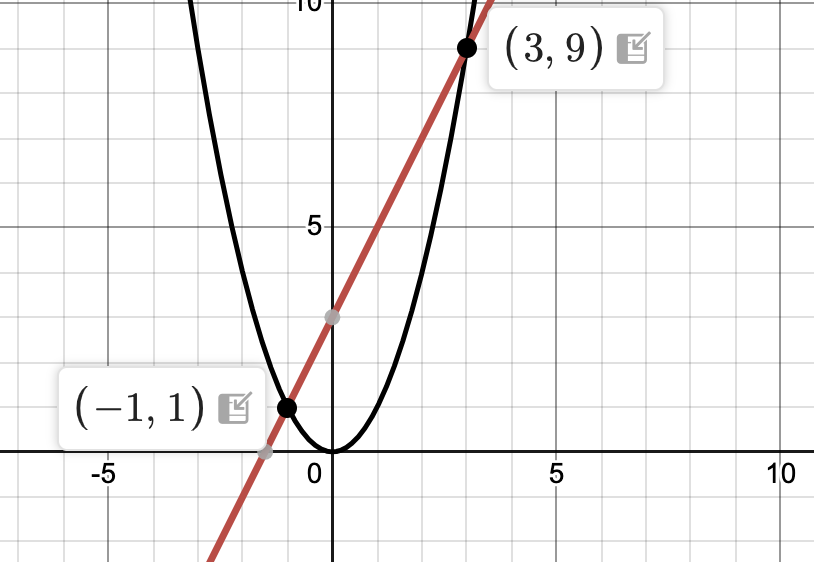
\includegraphics[width=0.4\linewidth]{E80.png}
  \end{center}
\end{frame}

\begin{frame}{Exactly One Real Solution}
  \textbf{Given the system:}
  \[
  \begin{cases}
  y = -1.5 \\
  y = x^2 + 8x + a
  \end{cases}
  \]

  \vspace{1em}
  \textbf{Question:} If the system has \textbf{exactly one real solution}, what is the value of $a$?
  \pause

  \vspace{1em}
  \textbf{Step 1:} Set the two equations equal to each other:
  \[
  x^2 + 8x + a = -1.5
  \Rightarrow x^2 + 8x + (a + 1.5) = 0
  \]

  \textbf{Step 2:} For a quadratic to have exactly one real solution, the discriminant must be zero:
  \[
  b^2 - 4ac = 0
  \Rightarrow 8^2 - 4(1)(a + 1.5) = 0
  \]

  \textbf{Step 3:} Solve:
  \[
  64 - 4(a + 1.5) = 0
  \Rightarrow a + 1.5 = 16
  \Rightarrow a = 14.5
  \]

  \vspace{0.5em}
  \textbf{Answer:} \boxed{14.5}
\end{frame}








\begin{frame}
\section{Vieta’s Theorem}
    \begin{tikzpicture}[remember picture, overlay]

        \shade[top color=softPurple, bottom color=softGray] 
            (current page.north west) rectangle (current page.south east);

        \fill[white, opacity=0.3] (current page.center) circle (4cm);
        

        \node[align=center] at (current page.center) {
            {\LARGE\bfseries\textcolor{purpleblue}{Vieta's Theorem}} \\[0.5cm]
            {\Large\itshape\textcolor{lightText}{Excellence in SAT Prep}}
        };
        \foreach \x in {1,2,3,4,5} {
            \fill[purpleblue, opacity=0.2] (rand*10-5, rand*7-3.5) circle (0.1+\x*0.05);
        }
        ;
    \end{tikzpicture}
\end{frame}

\begin{frame}{Vieta's Theorem for Quadratic Equations}
\textbf{Given:} A quadratic equation in standard form
\[
ax^2 + bx + c = 0
\]
with roots $r_1$ and $r_2$.

\vspace{0.3cm}
\textbf{Vieta's Theorem:}
\begin{itemize}
    \item Sum of the roots: $r_1 + r_2 = -\dfrac{b}{a}$
    \item Product of the roots: $r_1 \cdot r_2 = \dfrac{c}{a}$
\end{itemize}

\vspace{0.3cm}
\textbf{Why is this useful?}
\begin{itemize}
    \item Solve problems involving the relationships between roots without solving the equation.
    \item Helps in constructing quadratics from given roots.
\end{itemize}
\end{frame}

\begin{frame}{\textbf{Question: Sum of the Solutions of a Quadratic Equation}}
What is the sum of the solutions to the given equation?
\[
x^2 - 40x - 10 = 0
\]

\textbf{Options:}
\begin{enumerate}
    \item[A.] \(0\)
    \item[B.] \(5\)
    \item[C.] \(10\)
    \item[D.] \(40\)
\end{enumerate}
\end{frame}
\begin{frame}{\textbf{Answer Explanation: Sum of the Solutions}}
We are given a quadratic equation:
\[
x^2 - 40x - 10 = 0
\]

For any quadratic equation of the form:
\[
ax^2 + bx + c = 0,
\]
the sum of the solutions is given by the formula:
\[
\text{Sum} = -\frac{b}{a}.
\]

Here, \(a = 1\), \(b = -40\). Thus,
\[
\text{Sum} = -\frac{-40}{1} = 40.
\]

\textbf{Final Answer:} \(\boxed{40}\)
\end{frame}


\begin{frame}{\textbf{Question: Quadratic Product of Roots and Constants}}
In the given equation:
\[
57x^2 + (57b + a)x + ab = 0,
\]
where \(a\) and \(b\) are positive constants, the product of the solutions is given by \(kab\), where \(k\) is a constant.

\textbf{What is the value of } \(k\)?

\vspace{0.5cm}
\textbf{Options:}
\begin{enumerate}
    \item[A.] \(\frac{1}{57}\)
    \item[B.] \(\frac{1}{19}\)
    \item[C.] \(1\)
    \item[D.] \(57\)
\end{enumerate}
\end{frame}



\begin{frame}{\textbf{Answer Explanation: Product of Solutions}}
We are given the quadratic:
\[
57x^2 + (57b + a)x + ab = 0.
\]

Using the quadratic formula properties, the product of the roots of
\[
Ax^2 + Bx + C = 0
\]
is:
\[
\frac{C}{A}.
\]

So here:
\[
\text{Product of roots} = \frac{ab}{57}.
\]

We are told this equals \(kab\), so:
\[
kab = \frac{ab}{57}.
\]

\textbf{Final Answer:} \(\boxed{\frac{1}{57}}\)
\end{frame}




\begin{frame}
\section{Application}
    \begin{tikzpicture}[remember picture, overlay]

        \shade[top color=softPurple, bottom color=softGray] 
            (current page.north west) rectangle (current page.south east);

        \fill[white, opacity=0.3] (current page.center) circle (4cm);
        

        \node[align=center] at (current page.center) {
            {\LARGE\bfseries\textcolor{purpleblue}{Application}} \\[0.5cm]
            {\Large\itshape\textcolor{lightText}{Excellence in SAT Prep}}
        };
        \foreach \x in {1,2,3,4,5} {
            \fill[purpleblue, opacity=0.2] (rand*10-5, rand*7-3.5) circle (0.1+\x*0.05);
        }
        ;
    \end{tikzpicture}
\end{frame}


\begin{frame}{Application of Quadratic Functions}
\textbf{Real-World Example: Projectile Motion}

\vspace{0.2cm}
The height $h$ (in meters) of a ball thrown into the air after $t$ seconds is modeled by a quadratic function:
\[
h(t) = -4.9t^2 + vt + h_0
\]
where:
\begin{itemize}
    \item $-4.9$ is the acceleration due to gravity (in m/s\textsuperscript{2}),
    \item $v$ is the initial velocity (in m/s),
    \item $h_0$ is the initial height (in meters).
\end{itemize}

\vspace{0.3cm}
\textbf{Key Features:}
\begin{itemize}
    \item The \textbf{maximum height} occurs at the vertex.
    \item The \textbf{time to reach the ground} is when $h(t) = 0$ (solve the equation).
\end{itemize}

\vspace{0.3cm}
\textbf{Application:} Use quadratic equations to model and solve problems involving motion, area, and economics.
\end{frame}


\begin{frame}{\textbf{Question: Understanding Intercepts in a Revenue Function}}
\small
    The revenue \( f(x) \), in dollars, that a company receives from sales of a product is given by the function:
    \[
    f(x) = -500x^2 + 25{,}000x,
    \]
    where \(x\) is the unit price, in dollars, of the product.

    \vspace{0.3cm}
    The graph of \( y = f(x) \) in the \(xy\)-plane intersects the \(x\)-axis at \(0\) and \(a\).

    \vspace{0.3cm}
    What does \(a\) represent?

    \vspace{0.5cm}
    \textbf{Options:}
    \begin{enumerate}
        \item[A] The revenue, in dollars, when the unit price of the product is \$0
        \item[B] The unit price, in dollars, of the product that will result in maximum revenue
        \item[C] The unit price, in dollars, of the product that will result in a revenue of \$0
        \item[D] The maximum revenue, in dollars, that the company can make
    \end{enumerate}
\end{frame}

\begin{frame}{\textbf{Answer Explanation: Understanding Intercepts in a Revenue Function}}
    \textbf{Correct Answer: \textcolor{novelGreen}{C: The unit price, in dollars, of the product that will result in a revenue of \$0}}

    \vspace{0.3cm}
    \textbf{Explanation:}
    \begin{itemize}
        \item The function is a downward-opening parabola (\(a = -500 < 0\)).
        \item The \(x\)-intercepts of the graph represent values of \(x\) for which \(f(x) = 0\), meaning revenue is \$0.
        \item At \(x = 0\), revenue is 0 — this makes sense because selling at \$0 means no money is made.
        \item At \(x = a\), the company again makes \$0 revenue — likely because the price is too high and no one buys it.
        \item Thus, \(a\) represents the price at which the revenue becomes zero again.
    \end{itemize}

    \textbf{Final Answer:} \( \boxed{\text{C}} \)
\end{frame}


\begin{frame}{\textbf{Question: Interpreting the Vertex of a Quadratic Function in Context}}
The function 
\[
f(x) = \frac{1}{9}(x - 7)^2 + 3
\]
gives a metal ball's height above the ground \(f(x)\), in inches, \(x\) seconds after it started moving on a track, where \(0 \leq x \leq 10\). 

Which of the following is the best interpretation of the vertex of the graph of \(y = f(x)\) in the \(xy\)-plane?

\vspace{0.4cm}
\textbf{Options:}
\begin{enumerate}
    \item[A] The metal ball's minimum height was 3 inches above the ground.
    \item[B] The metal ball's minimum height was 7 inches above the ground.
    \item[C] The metal ball's height was 3 inches above the ground when it started moving.
    \item[D] The metal ball's height was 7 inches above the ground when it started moving.
\end{enumerate}
\end{frame}

\begin{frame}{\textbf{Answer Explanation: Vertex of a Quadratic in Real-World Context}}
\textbf{Correct Answer: \textcolor{novelGreen}{A: The metal ball's minimum height was 3 inches above the ground.}}

\vspace{0.3cm}
\textbf{Explanation:}
\begin{itemize}
    \item The function is written in vertex form: \(f(x) = a(x - h)^2 + k\), where the vertex is at \((h, k)\).
    \item Here, the vertex is at \((7, 3)\).
    \item Since the coefficient of the squared term is positive \(\left(\frac{1}{9}\right)\), the parabola opens upward, and the vertex represents a minimum.
    \item So, the ball reaches its \textbf{minimum height} of 3 inches \textbf{7 seconds} after it starts moving.
\end{itemize}

\textbf{Final Answer:} \( \boxed{\text{A}} \)
\end{frame}



\begin{frame}
\section{Practices}
    \begin{tikzpicture}[remember picture, overlay]

        \shade[top color=softPurple, bottom color=softGray] 
            (current page.north west) rectangle (current page.south east);

        \fill[white, opacity=0.3] (current page.center) circle (4cm);
        

        \node[align=center] at (current page.center) {
            {\LARGE\bfseries\textcolor{purpleblue}{Practices
        }} \\[0.5cm]
            {\Large\itshape\textcolor{lightText}{Excellence in SAT Prep}}
        };
        \foreach \x in {1,2,3,4,5} {
            \fill[purpleblue, opacity=0.2] (rand*10-5, rand*7-3.5) circle (0.1+\x*0.05);
        }
        ;
    \end{tikzpicture}
\end{frame}



\begin{frame}{Question}
The function $f(x) = 3x^2 + bx + c$ is a quadratic function, where $b$ and $c$ are constants.

The graph of $y = f(x)$ in the $xy$-plane does not intersect the $x$-axis. If $f(-7) = f(9)$, which of the following could be the value of $b + c$?

\begin{enumerate}
  \item[A)] $-1$
  \item[B)] $-3$
  \item[C)] $-5$
  \item[D)] $-7$
\end{enumerate}
\end{frame}


\begin{frame}{Answer I}
We are given:
\[
f(x) = 3x^2 + bx + c, \quad f(-7) = f(9)
\]

Use symmetry: $f(-7) = f(9)$ implies that the axis of symmetry is the midpoint between $-7$ and $9$:

\[
x = \frac{-7 + 9}{2} = 1
\Rightarrow \text{Vertex is at } x = 1
\]

The vertex of a quadratic $f(x) = ax^2 + bx + c$ occurs at:
\[
x = -\frac{b}{2a} = -\frac{b}{6}
\]

Set equal to 1:
\[
-\frac{b}{6} = 1 \Rightarrow b = -6
\]

Now plug $b = -6$ into the original function:
\[
f(x) = 3x^2 - 6x + c
\]

\end{frame}
\begin{frame}{Answer II}

Now compute $b + c = -6 + c$, and check answer choices.

Try:
- A) $-1 \Rightarrow c = 5$
- B) $-3 \Rightarrow c = 3$
- C) $-5 \Rightarrow c = 1$
- D) $-7 \Rightarrow c = -1$

We also know the graph does not intersect the $x$-axis → discriminant $< 0$:
\[
\Delta = b^2 - 4ac = (-6)^2 - 4(3)(c) = 36 - 12c
\]

We want $36 - 12c < 0 \Rightarrow c > 3$

Only option that gives $c > 3$ is:

\[
\boxed{A) \ -1 \Rightarrow b + c = -6 + 5 = -1}
\]

\textbf{Correct answer:} A
\end{frame}



\begin{frame}{\textbf{Question: Properties of a Quadratic Function}}
The function is given as:
\[
f(x) = ax^2 + 4x + c
\]
where \(a\) and \(c\) are constants. The parabola opens upward and has a vertex at point \((h, k)\). It is also given that:
\begin{itemize}
    \item \(k < 0\)
    \item \(f(-9) = f(3)\)
\end{itemize}

Which of the following must be true?

\begin{enumerate}
    \item[\textbf{I.}] \(c < 0\)
    \item[\textbf{II.}] \(a \geq 1\)
\end{enumerate}

\vspace{0.1cm}
\textbf{Options:}
\begin{enumerate}
    \item[A]  I only
    \item[B] II only
    \item[C] I and II
    \item[D] Neither I nor II
\end{enumerate}
\end{frame}


\begin{frame}{\textbf{Answer Explanation: Use of Symmetry and Vertex}}
We are told:
\[
f(x) = ax^2 + 4x + c
\quad \text{and} \quad f(-9) = f(3)
\]

\textbf{Step 1: Use symmetry of a parabola.}  
If \(f(-9) = f(3)\), then these points are symmetric about the vertex.

So, the axis of symmetry (i.e. x-value of vertex) is:
\[
x = \frac{-9 + 3}{2} = -3
\]

\textbf{Step 2: Use vertex formula to confirm.}  
The x-coordinate of the vertex of a quadratic is given by:
\[
x = \frac{-b}{2a}
\]
Here, \(f(x) = ax^2 + 4x + c\), so:
\[
\frac{-4}{2a} = -3 \Rightarrow a = \frac{2}{3}
\]


\end{frame}

\begin{frame}{Answer Explanation: Use of Symmetry and Vertex}

Thus, statement II: \(a \geq 1\) is \textbf{not necessarily true.}

\vspace{0.3cm}
\textbf{Step 3: What about } \(c < 0\)?  
From the question, we know that \textbf{$k <0$}. Therefor, by using \textbf{Vertex Formula} \[
\frac{4ac-b^2}{4a}<0
\] , we can get that $c<6$. Hence, Option II is wrong

\vspace{0.3cm}
\textbf{Final Answer:} \(\boxed{\text{D. Neither I nor II}}\)
    
\end{frame}

\begin{frame}{\textbf{Question: Parabola Vertex and Coefficient Sum}}
In the \(xy\)-plane, a parabola has vertex \( (9, -14) \) and intersects the \(x\)-axis at two points.  
If the equation of the parabola is written in the form:
\[
y = ax^2 + bx + c,
\]
where \(a\), \(b\), and \(c\) are constants, which of the following could be the value of \(a + b + c\)?

\vspace{0.3cm}
\textbf{Options:}
\begin{enumerate}
    \item [A] \(-23\)
    \item [B] \(-19\)
    \item [C] \(-14\)
    \item [D] \(-12\)
\end{enumerate}
\end{frame}


\begin{frame}{\textbf{Answer Explanation: Convert from Vertex to Standard Form}}
We are given:
\begin{itemize}
    \item Vertex: \( (9, -14) \)
    \item Parabola intersects the \(x\)-axis at two points \( \Rightarrow \) it opens upwards or downwards (not a single point).
\end{itemize}

\textbf{Step 1: Use vertex form.}
\[
y = a(x - 9)^2 - 14
\]

\textbf{Step 2: Expand to standard form.}
\[
y = a(x^2 - 18x + 81) - 14 = ax^2 - 18a x + 81a - 14
\]

So we identify:
\[
a = a, \quad b = -18a, \quad c = 81a - 14
\]

\textbf{Step 3: Compute the sum \(a + b + c\):}
\[
a + (-18a) + (81a - 14) = (a - 18a + 81a) - 14 = 64a - 14
\]


\end{frame}


\begin{frame}{\textbf{Question: System of Equations - One Point of Intersection}}
Given the system of equations:
\[
y = 2x^2 - 21x + 64
\]
\[
y = 3x + a
\]

In the system, \(a\) is a constant. The graphs intersect at exactly one point \((x, y)\) in the \(xy\)-plane. What is the value of \(x\)? 

(\textbf{Can you do this question without using Quadratic Formula ?})

\vspace{0.2cm}
\textbf{Options:}
\begin{enumerate}
    \item[A.] \(-8\)
    \item[B.] \(-6\)
    \item[C.] \(6\)
    \item[D.] \(8\)
\end{enumerate}
\end{frame}


\begin{frame}{\textbf{Answer I}}
\small
We set the two expressions for \(y\) equal:
\[
2x^2 - 21x + 64 = 3x + a
\]

Move all terms to one side:
\[
2x^2 - 24x + (64 - a) = 0
\]

Since the graphs intersect at exactly one point, this quadratic must have exactly one solution. That means the discriminant is zero:
\[
\Delta = b^2 - 4ac = 0
\]

Here, \(a = 2\), \(b = -24\), \(c = 64 - a\). So:
\[
(-24)^2 - 4(2)(64 - a) = 0
\]
\[
576 - 8(64 - a) = 0
\Rightarrow 576 - 512 + 8a = 0
\Rightarrow 64 + 8a = 0 \Rightarrow a = -8
\]

Now substitute \(a = -8\) into the original system:
\[
y = 3x - 8
\quad \text{and} \quad
y = 2x^2 - 21x + 64
\]


\end{frame}
\begin{frame}{Answer II}
    Set equal again:
\[
2x^2 - 21x + 64 = 3x - 8
\Rightarrow 2x^2 - 24x + 72 = 0
\]

Divide by 2:
\[
x^2 - 12x + 36 = 0
\Rightarrow (x - 6)^2 = 0 \Rightarrow \boxed{x = 6}
\]

\textbf{Final Answer: C. \(6\)}

\end{frame}


\begin{frame}{Question}
The function 
\[
f(x) = a(x - 3)(x - k)
\]
is a quadratic, where $a$ and $k$ are constants.

The graph of $y = f(x)$ in the $xy$-plane is a parabola with vertex $(5, -32)$. What is the value of $a$?

\begin{enumerate}
  \item[A)] 2
  \item[B)] 5
  \item[C)] 6
  \item[D)] 8
\end{enumerate}
\end{frame}

\begin{frame}{Answer}
Given: $f(x) = a(x - 3)(x - k)$ and vertex is at $(5, -32)$.

Step 1: Use symmetry — the $x$-coordinate of the vertex is the midpoint of the roots:

\[
\frac{3 + k}{2} = 5 \Rightarrow 3 + k = 10 \Rightarrow k = 7
\]

So the function is:
\[
f(x) = a(x - 3)(x - 7)
\]

Step 2: Plug in the vertex point $(5, -32)$:
\[
f(5) = a(5 - 3)(5 - 7) = a(2)(-2) = -4a
\]

\[
-4a = -32 \Rightarrow a = 8
\]

\textbf{Correct answer:} D
\end{frame}






\begin{frame}{}
    \begin{tikzpicture}[remember picture, overlay]
        % 背景渐变色：蓝紫到白
        \shade[top color=novelPurple!40, bottom color=white]
            (current page.north west) rectangle (current page.south east);

        % 中心柔光
        \fill[white, opacity=0.15] (current page.center) circle (5cm);

        % 柔和光点点缀
        \foreach \x in {1,2,3,4,5} {
            \fill[novelPurple, opacity=0.12] (rand*10-5, rand*7-3.5) circle (0.1+\x*0.05);
        }
    \end{tikzpicture}

    \centering
    \vspace{5em}

    {\Huge \textbf{\textcolor{novelPurple}{Thank You!}}} \\[1em]
    {\large \textcolor{gray}{We appreciate your time and focus.}} \\[3em]

    {\LARGE \textbf{\textcolor{novelPurple}{\textsf{Novel Prep}}}}

    \vfill
\end{frame}













\end{document}
